\documentclass[a4paper,11pt]{article}
\usepackage[utf8]{inputenc}
\usepackage{lastpage}
\usepackage{fancyhdr}
\usepackage[english]{babel}
\usepackage[a4paper,margin=1in]{geometry}
\usepackage{multirow}
\usepackage[table,xcdraw]{xcolor}
\usepackage{array}
\usepackage{graphicx}
\usepackage{caption}
\usepackage{ctable}
\usepackage{listings}
\usepackage[T1]{fontenc}
\usepackage{bigfoot} % to allow verbatim in footnote
\usepackage[numbered,framed]{matlab-prettifier}
\usepackage{amsmath}


\newcolumntype{L}[1]{>{\raggedright\let\newline\\\arraybackslash\hspace{0pt}}m{#1}}
\newcolumntype{C}[1]{>{\centering\let\newline\\\arraybackslash\hspace{0pt}}m{#1}}
\newcolumntype{R}[1]{>{\raggedleft\let\newline\\\arraybackslash\hspace{0pt}}m{#1}}

\newcommand\tab[1][4mm]{\hspace*{#1}}


%-------------------------------------------------------------------------------
% HEADER & FOOTER
%-------------------------------------------------------------------------------

\pagestyle{fancy}
\fancyhf{}
\setlength\headheight{15pt}
\fancyhead[L]{ Imaging Lab 11 }
\fancyhead[R]{Student ID: 100633486}
\fancyfoot[R]{Page \thepage\ of \pageref{LastPage}}


%-------------------------------------------------------------------------------
% TITLE PAGE
%-------------------------------------------------------------------------------

\begin{document}

\title{
	\Huge \textbf {Image Registration}
    \\ [0.2cm]
	\LARGE Imaging Lab 11 - May, 2017
    \\ [0.5cm]
    \hrule
}

\date{}

\author{
		\Large Kamyar Nazeri \\
		\large Student ID: 100633486 }

\maketitle
\newpage

\section*{Image Morphing}
Morphing is a special effect in motion pictures and animations that changes (or morphs) one image or shape into another through a seamless transition. Traditionally such a depiction would be achieved through cross-fading techniques; we are using image registration while also performing a cross-dissolve to gradually transform one image into another and create more realistic transition. \\\\
We select corresponding control points in both images using Matlab's \emph{cpselect} tool:

\begin{lstlisting}[
    style=Matlab-editor,
    numbers=none,
    frame=none,
    xleftmargin=.2in
]
cpselect (A, B);
\end{lstlisting}
 \\
And click on 4 corresponding pairs of points: the left eye, right eye, tip of the nose, and bottom of the chin (\emph{Figure 1}):

\begin{figure}[!htb]
  \centering
  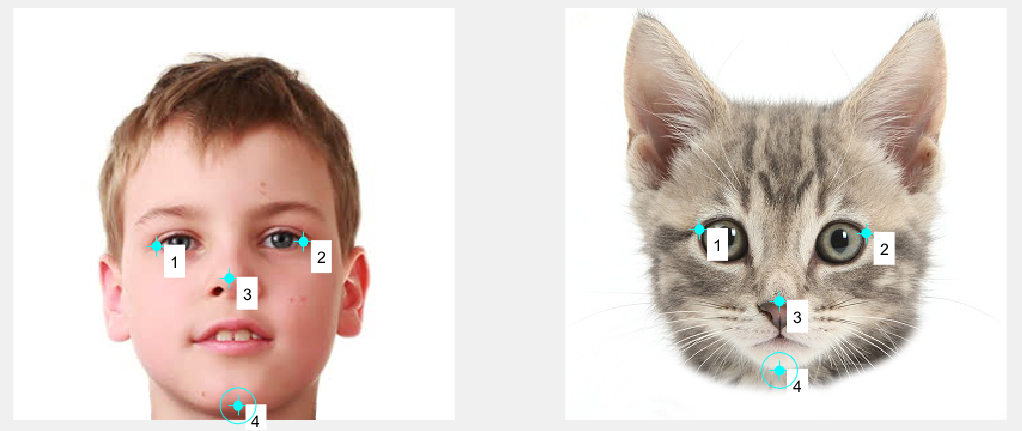
\includegraphics[width=14cm, height=5.9cm]{2.png}
  \caption{\small Selecting control points in both images using Matlab's cpselect tool.}
\end{figure}

 \\
Now we can gradually warp the image A to B by performing a weighted average of these control points. \emph{Figure 2} shows the result image morphing on every 20th frame of the transformation:

\begin{figure}[!htb]
  \centering
  
\includegraphics[width=14cm, height=7.4cm]{1.png}
  \caption{\small Image morphing on every 20th frame of the transformation.}
\end{figure}

\newpage
\section*{Coding Image Morphing}
\emph{Listing 1} shows the Feature-Based Image Registration technique used to transform one image into another. Note that control points in the images are chosen by the user: \\
\begin{lstlisting}[caption={Image registration technique used to transform image A into image B},captionpos=b,style=Matlab-editor]
A = imread('1.png');
B = imread('2.png');

[m,n,k] = size(B);      % get reference image size
A = imresize(A,[m,n]);  % make the two images the same size
cpselect (A, B);        % select control points in both images

for t=0:0.01:1
    % gradually warp the image A to B by
    % performing weighted average of the control points
    P_mid = (1-t)*PA + t*PB;
    
    % affine transformation that maps the points PA to P_mid         
    T_mid = cp2tform(PA, P_mid, 'affine');
    
    % put both images on the same coordinate system
    [A_T, B_T] = align (A, B, T_mid);
    
    % cross-fade between two aligned images
    I = (1-t)*A_T + t*B_T;

    if mod(t,0.2) == 0
        subplot(2,3,1+5*t);
        imagesc(I); axis image off; drawnow;
    end;
end;

\end{lstlisting}



\end{document}
